\mychapter{Expression des besoins}

\section{Introduction}
Dans ce chapitre se concentre sur l'expression et l'analyse des besoins de notre système.
Dans un premier temps, nous identifions les divers acteurs qui interagissent avec le systéme
puis les besoins fonctionnels, non fonctionnels et les besoins décisionnels qui sont répertoriés dans notre système.
Enfin, nous élaborons ces besoins par des  spécifications détaillées des cas d'utilisation, présentée par un diagramme  de cas d'utilisation raffiné
\section{Identifications des acteurs}

Un acteur est une abstraction d'un rôle joué par les utilisateurs du système pouvant être une personne ou un autre système qui interagissent directement avec le système à modéliser.

Notre système est utilisé par deux acteurs :CEO (l'administrateur) et l'agent commercial.

\subsection*{CEO(Admin)}

C'est le propriétaire du dépôt de boissons, il détient le niveau d'accès le plus élevé du système.

Il bénéficie d'un accès global lui permettant de gérer l'ensemble des opérations.

Il est responsable de la gestion des comptes utilisateurs.

Il assure également le suivi des données stratégiques de l'entreprise (produits « boissons », clients, ventes, facturation et paiements) afin de prendre des décisions pertinentes et éclairées.

\subsection*{Agent commercial}

L'agent commercial est responsable de la gestion opérationnelle des activités de vente au quotidien.

Il assure le bon déroulement du processus de vente, la bonne gestion des clients et des boissons, générer des factures ainsi que la validation des paiements.

Il s'occupe également de la consultation et de l'impression des factures et de l'envoi via whatsapp

\section{Identification des besoins}

\subsection{Identification des besoins fonctionnels}
\begin{itemize}


\item \textbf{Se connecter :} Permet à l'agent commercial et CEO d'accéder au système en saisissant ses identifiants (email et mot de passe) afin d'accéder aux fonctionnalités autorisées.

\item \textbf{Gérer Produit :} Permet à l'agent commercial et au CEO d'ajouter, modifier, consulter, archiver et supprimer uniquement les boissons qui ne sont pas encore associées à une vente

\item \textbf{Gérer client:} Permet à l'agent commercial et au CEO d'ajouter, modifier, archiver, consulter les informations relatives aux clients et les supprimer uniquement s'ils ne sont pas encore associés à une vente.

\item \textbf{Traiter vente :} Permet à l'agent commercial et au CEO d'enregistrer les nouvelles ventes, de suivre leur état, de consulter l'historique des ventes et d'effectuer l'archivage d'une vente.

\item \textbf{Gérer Facture :} permet à l'agent commercial et au CEO de créer, consulter, archiver, enregistrer un règlement ainsi que de suivre les détails de paiement (mode, type, montant payé, date de paiement et date d'échéance) avec la possibilité de l'imprimer ou de l'envoyer via WhatsApp.

\item \textbf{Gérer Agent commercial :} Permet au CEO d'ajouter et de supprimer les agents commerciaux qui utilisent le système 

\item \textbf{Gérer Notification :} Permet au CEO et à l'agent commercial d'être informés en temps réel des événements critiques du système (tels que la rupture de stock d'un produit, la date d'échéance d'un règlement arrivant aujourd'hui etc.) 

Ils ont la possibilité de les marquer comme lues ou de les supprimer s'ils n'en ont plus besoin.

\item \textbf{Consulter les tableaux de bord :} Permet au CEO de visualiser les indicateurs clés de performance (KPI) et les statistiques des ventes sous forme de graphiques.

\item \textbf{Consulter les prévisions des ventes :} Permet au CEO de visualiser les prévisions des ventes futures, basées sur les données historiques des ventes, afin d'aider à la prise de décision stratégique.

\end{itemize}
\newpage


\begin{figure}[H]
  \centering
  \makebox[\textwidth][c]{%
    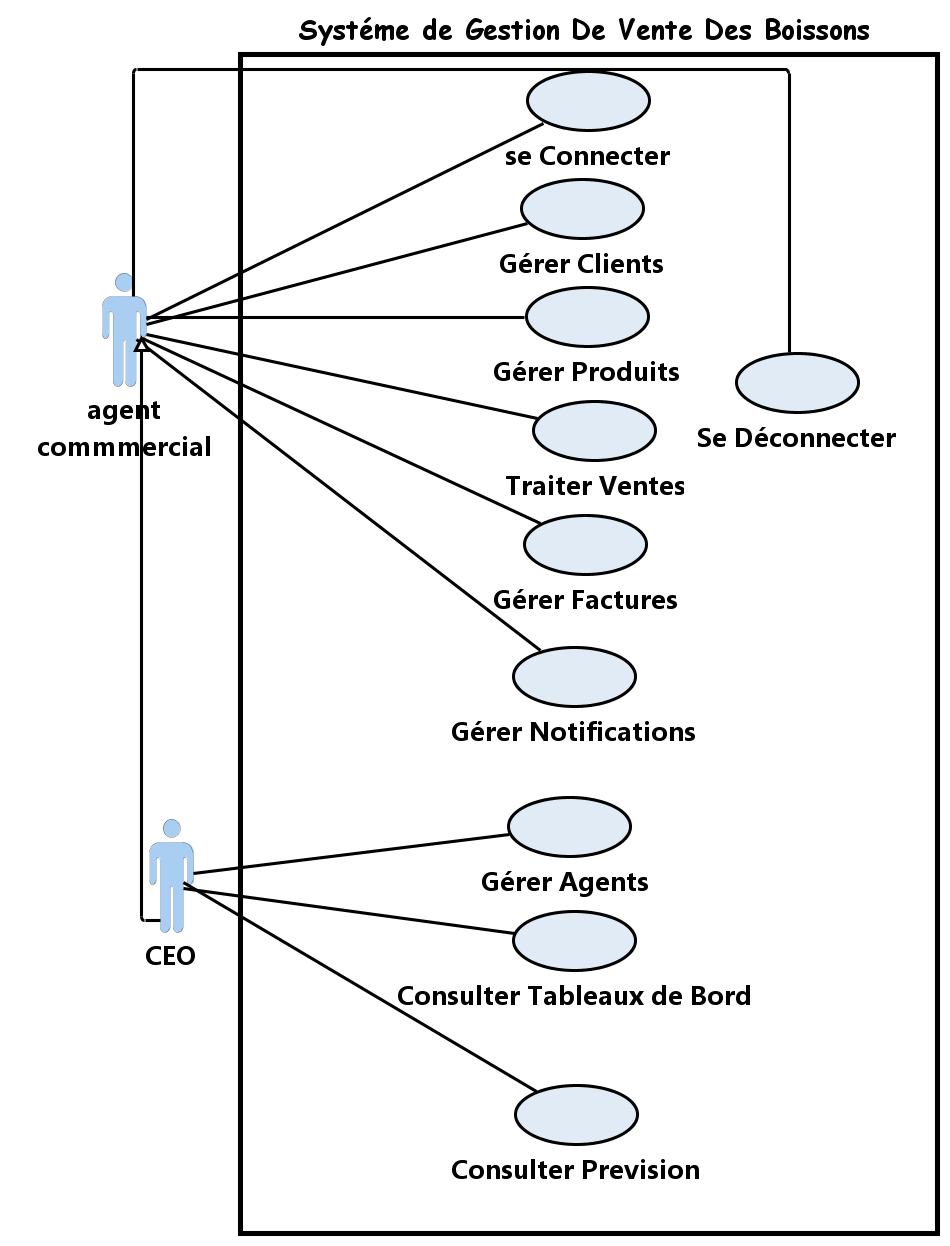
\includegraphics[width=1.2\textwidth, height=0.93\textheight]{images/MCU_DiagrammeCasUtilisationGlobal.png}%
  }
  \caption{Diagramme de cas d'utilisation globale}
  \label{fig:usecaseglobal}
\end{figure}

\newpage


\section{Identification des besoins non fonctionnels}

\begin{itemize}

\item \textbf{Sécurité :} le système protège les données des utilisateurs ainsi que les informations privilégiées (telles que les informations liées aux clients, aux ventes et aux factures).

\item \textbf{Fiabilité :} le système est capable de fonctionner d'une manière efficace, sans erreur.

\item \textbf{Ergonomie :} notre système est clair, avec une interface simple, compréhensible et intuitive. Il est également facile à utiliser.

\item \textbf{Maintenabilité :} le système est capable d'être modifié ou amélioré même après son implémentation, sans perturber l'exécution des fonctionnalités existantes.

\end{itemize}



\section{Identification des besoins décisionnels}

\subsection*{Les besoins décisionnels du CEO (Admin)}

\begin{itemize}

\item \textbf{Le suivi global des opérations du système}

Le système permet d'assurer le suivi global des opérations en mettant à disposition des données complètes et détaillées, notamment les informations relatives aux ventes, aux produits, aux factures, aux clients, aux paiements ainsi qu'aux utilisateurs du système. Cette vision globale permet au CEO de suivre et de contrôler l'ensemble des opérations afin d'assurer une gestion efficace du système.

\item \textbf{Gestion des risques}

Le système permet au CEO de détecter les anomalies liées aux transactions et au stock, notamment les ventes non réglées, les paiements au comptant ou partiels, ainsi que les anomalies concernant les produits finis en stock, afin d'assurer une prise de décision efficace et de garantir la fiabilité des opérations de ventes.

\item \textbf{Les décisions stratégiques}

Le système met à disposition du CEO des tableaux de bord stratégiques offrant une vision claire et synthétique de la situation de l'entreprise. Ces outils permettent d'identifier les produits les plus performants, les clients les plus actifs et les clients fidèles, de suivre le volume des ventes par période, le chiffre d'affaires ainsi que la répartition des paiements (au comptant ou à crédit).

Le système offre également des tableaux de prévision des ventes, permettant d'anticiper l'évolution future de l'activité à partir des données historiques.

\end{itemize}
\newpage

\section{Affectation des priorités aux cas d'utilisation}

Afin de faciliter la planification et le développement du système, nous avons attribué un niveau de priorité à chaque cas d'utilisation selon son importance dans le fonctionnement global de l'application.

Les fonctionnalités essentielles au démarrage et au bon déroulement des opérations quotidiennes ont été classées avec une priorité élevée, tandis que les fonctionnalités d'analyse, de prévision et de confort d'utilisation ont été placées à des niveaux de priorité inférieurs.

Le tableau suivant présente l'ensemble des cas d'utilisation ainsi que leur niveau de priorité.

\begin{table}[H]
\centering

\renewcommand{\arraystretch}{1.2}



\begin{tabular}{|p{9cm}|c|}
\hline
\rowcolor{purple!25}
\textbf{Cas d'utilisation} & \textbf{Priorité} \\
\hline
Se connecter & 1 \\
\hline
Gérer Produit & 1 \\
\hline
Gérer Clients & 1 \\
\hline
Gérer Agents & 1 \\
\hline
Traiter Ventes & 2 \\
\hline
Gérer Factures & 2 \\
\hline
Consulter les Tableaux de Bord & 3 \\
\hline
Consulter Prévisions & 4 \\
\hline
Gérer Notifications & 5 \\
\hline
Se Déconnecter & 5 \\
\hline
\end{tabular}

\caption{Priorité des cas d'utilisation}

\end{table}

\newpage
\section{Spécification et raffinement des cas d'utilisation}

\subsection{Spécification du cas d'utilisation Se Connecter}

\begin{table}[H]
\begin{tabularx}{\textwidth}{|l|X|}
\hline
\textbf{Titre CU :} & Se Connecter \\
\hline
\textbf{Acteur(s) :} & Agent commercial, CEO \\
\hline
\textbf{Description brève :} & Ce cas d'utilisation permet aux acteurs de se connecter afin d'accéder à leurs espaces de travail \\
\hline
\textbf{Postcondition(s)} & L'utilisateur est connecté avec succès \\
\hline
\textbf{Scénario de base :} &
\begin{enumerate}[leftmargin=1.5em, topsep=2pt, itemsep=1pt]
  \item L'utilisateur accède à la page de connexion
  \item Le système permet à l'utilisateur d'entrer son email et mot de passe
  \item L'utilisateur confirme son identification
  \item Le système vérifie la validité des information remplies
  \item Le système confirme que l'utilisateur existe et que le mot de passe correcte
  \item Le système ouvre l'espace de travail correspondant à chaque utilisateur
\end{enumerate} \\
\hline
\textbf{Autre(s) scénario(s)} &
\textbf{4.a. information obligatoires manquantes ou invalide}
\begin{enumerate}[leftmargin=1.5em, topsep=2pt, itemsep=1pt]
  \item Le système informe l'agent qu'il y a des informations obligatoires manquants
  \item Le système retourne à l'étape 2 du scénario de base
\end{enumerate}
\textbf{4.b. e-mail ou un mot de passe non reconnu}
\begin{enumerate}[leftmargin=1.5em, topsep=2pt, itemsep=1pt]
  \item Le système informe l'utilisateur que son email ou son mot de passe sont incorrecte
  \item Le système retourne à l'étape 2 de scénario de base
\end{enumerate} \\
\hline
\end{tabularx}
\caption{Spécification du CU : Se Connecter}
\label{tab:cu-connecter}
\end{table}

\newpage
\subsection{Spécification du cas d'utilisation Se Déconnecter}

\begin{table}[H]
\begin{tabularx}{\textwidth}{|l|X|}
\hline
\textbf{Titre CU :} & se Déconnecter \\
\hline
\textbf{Acteur(s) :} & Agent commercial, CEO \\
\hline
\textbf{Description brève :} & Ce cas d'utilisation permet aux acteurs de se déconnecter de leur espace de travail \\
\hline
\textbf{Pré-condition(s)} & L'utilisateur est connecté \\
\hline
\textbf{Post-condition(s)} & L'utilisateur est déconnecté du système et redirigé vers la page de connexion \\
\hline
\textbf{Scénario de base :} &
\begin{enumerate}[leftmargin=1.5em, topsep=2pt, itemsep=1pt]
  \item L'utilisateur demande de se déconnecter
  \item Le système affiche la fenêtre de déconnexion
  \item Le système demande l'utilisateur de confirmer l'opération de déconnexion
  \item L'utilisateur confirme la déconnexion
  \item Le système redirige l'utilisateur vers la page de connexion
\end{enumerate} \\
\hline
\textbf{Autre(s) scénario(s)} &
\textbf{4a. L'utilisateur demande d'annuler la déconnexion}
\begin{enumerate}[leftmargin=1.5em, topsep=2pt, itemsep=1pt]
  \item Le système informe l'utilisateur que l'opération est annulée
  \item Le système reste dans l'espace de travail
  \item Le CU Se termine
\end{enumerate} \\
\hline
\end{tabularx}
\caption{Spécification du CU : Se Déconnecter}
\label{tab:cu-deconnecter}
\end{table}

\newpage
\section{Spécification de cas d'utilisation Gérer Agents}

\subsection{Spécification du cas d'utilisation Ajouter Agents}

\begin{table}[H]
\begin{tabularx}{\textwidth}{|l|X|}
\hline
\textbf{Titre CU :} & Ajouter Agents \\
\hline
\textbf{Acteur(s) :} & CEO \\
\hline
\textbf{Description brève :} & Ce cas d'utilisation permet au CEO d'ajouter un nouvel agent dans le système en renseignant son adresse email et son mot de passe. \\
\hline
\textbf{Pré-condition(s)} & Le CEO est connecté \\
\hline
\textbf{Post-condition(s)} & Le nouvel agent est enregistré \\
\hline
\textbf{Scénario de base :} &
\begin{enumerate}[leftmargin=1.5em, topsep=2pt, itemsep=1pt]
  \item Le CEO demande la gestion des agents
  \item Le CEO demande l'ajout d'un nouvel agent
  \item Le système affiche le formulaire d'ajout
  \item Le CEO fournit les informations liées à l'agent
  \item Le CEO demande d'enregistrer les détails de l'agent
  \item Le système vérifie si toutes les informations obligatoires sont remplies et sont valides
  \item Le système vérifie si l'email existe déjà
  \item Le système enregistre le nouvel agent
  \item Le système informe le CEO que l'agent est ajouté avec succès
  \item Le système affiche l'agent dans la liste
\end{enumerate} \\
\hline
\textbf{Autre(s) scénario(s)} &
\textbf{6.a informations obligatoires manquantes}
\begin{enumerate}[leftmargin=1.5em, topsep=2pt, itemsep=1pt]
  \item Le système détecte qu'il Ya des détails obligatoires manquantes
  \item Le système informe l'agent de remplir les informations manquantes
  \item Le système retourne à l'étape 4 du scénario de base
\end{enumerate}
\textbf{7.a Email déjà enregistré dans le système}
\begin{enumerate}[leftmargin=1.5em, topsep=2pt, itemsep=1pt]
  \item Le système informe le CEO que cet email existe déjà.
  \item Le CU se Termine.
\end{enumerate} \\
\hline
\end{tabularx}
\caption{Spécification du CU : Ajouter Agent}
\label{tab:cu-ajouter-agent}
\end{table}

\newpage
\subsection{Spécification du cas d'utilisation supprimer Agent}

\begin{table}[H]
\begin{tabularx}{\textwidth}{|l|X|}
\hline
\textbf{Titre CU :} & supprimer utilisateur \\
\hline
\textbf{Acteur(s) :} & CEO \\
\hline
\textbf{Description brève :} & Ce cas d'utilisation permet au CEO de supprimer un agent existant \\
\hline
\textbf{Pré-condition(s)} & Le CEO est connecté et au moins un agent existe dans le système \\
\hline
\textbf{Post-condition(s)} & L'agent est supprimé définitivement du système et ne peut plus se connecter \\
\hline
\textbf{Scénario de base :} &
\begin{enumerate}[leftmargin=1.5em, topsep=2pt, itemsep=1pt]
  \item Le CEO demande la page Agents
  \item le systéme cherche tous les agents existants
  \item Système affiche la liste des agents.
  \item Le CEO sélectionne l'agent à supprimer.
  \item Le CEO demande de supprimer l'agent sélectionner
  \item Le système demande une confirmation de suppression.
  \item Le CEO confirme la suppression.
  \item Le système supprime définitivement l'agent
  \item Le système informe le CEO que l'agent est supprimé avec succès.
\end{enumerate} \\
\hline
\textbf{Autre(s) scénario(s)} &
\textbf{6.a. suppression annuler}
\begin{enumerate}[leftmargin=1.5em, topsep=2pt, itemsep=1pt]
  \item Le CEO demande d'annuler la suppression de l'agent
  \item Le système informe le CEO que la suppression a été annuler
  \item Le CU se termine
\end{enumerate} \\
\hline
\end{tabularx}
\caption{Spécification du CU : Supprimer Agent}
\label{tab:cu-supprimer-agent}
\end{table}

\clearpage

\section{Spécification de cas d'utilisation Gérer produit}

\subsection{Spécification de cas d'utilisation Ajouter Produit}

\begingroup
\small
\renewcommand{\arraystretch}{0.92}
\begin{longtable}{|p{3.4cm}|p{11.2cm}|}
\hline
\textbf{Titre CU :} & Ajouter Produit \\
\hline
\textbf{Acteur(s) :} & Agent commercial \\
\hline
\textbf{Description brève :} & Ce cas d'utilisation permet à l'Agent commercial d'ajouter un nouveau produit (boisson gazeuse, jus, eau) en renseignant ses informations telles que le nom du produit, la catégorie, le prix unitaire, le prix d'achat et la quantité en stock. \\
\hline
\textbf{Pré-condition(s)} & L'Agent commercial est connecté \\
\hline
\textbf{Postcondition(s)} & Le produit est enregistré avec le statut disponible à la vente ou faible \\
\hline
\textbf{Scénario de base :} &
\begin{enumerate}[leftmargin=1.5em, topsep=2pt, itemsep=1pt]
  \item L'Agent commercial demande la gestion des produits
  \item L'Agent commercial demande Ajouter produit
  \item Le système permet à l'agent commercial d'entrer les détails d'un nouveau produit
  \item L'Agent commercial fournit les informations requises
  \item L'Agent commercial demande d'enregistrer tous les détails du produit
  \item Le système vérifie si toutes les informations obligatoires sont remplies et sont valides
  \item Le système vérifie si le produit existe déjà
  \item Le système affecte un état au produit en fonction de la valeur de stock introduite par l’agent
  \item Le système enregistre le produit à l'état disponible
  \item Le système informe l'agent que le produit est ajouté avec succès
\end{enumerate} \\
\hline
\textbf{Autre(s) scénario(s)} &
\textbf{6.a informations obligatoires non remplis et non valide :}
\begin{enumerate}[leftmargin=1.5em, topsep=2pt, itemsep=1pt]
  \item Le système informe l'agent de remplir les informations manquantes
  \item Le système retourne à l'étape 4 du scénario de base
\end{enumerate}
\textbf{6.b quantite de stock = 0 :}
\begin{enumerate}[leftmargin=1.5em, topsep=2pt, itemsep=1pt]
  \item Le système informe l'agent que le stock doit être supérieur à 0
  \item Le système retourne à l'étape 4 du scénario de base
\end{enumerate}
\textbf{7.a Produit déjà enregistrer dans le système :}
\begin{enumerate}[leftmargin=1.5em, topsep=2pt, itemsep=1pt]
  \item Le système informe l'agent que le produit existe déjà
  \item Le CU se termine sans ajout d'un nouveau produit
\end{enumerate}
\textbf{9.a quantite de stock <= 5 :}
\begin{enumerate}[leftmargin=1.5em, topsep=2pt, itemsep=1pt]
  \item Le système enregistre le produit à l'état faible
\end{enumerate} \\
\hline
\caption{Spécification du CU : Ajouter Produit}
\label{tab:cu-ajouter-produit}
\end{longtable}
\endgroup

\newpage
\subsection{Spécification de cas d'utilisation supprimer produit}

\begin{table}[H]
\begin{tabularx}{\textwidth}{|l|X|}
\hline
\textbf{Titre CU :} & Supprimer produit \\
\hline
\textbf{Acteur(s) :} & Agent commercial \\
\hline
\textbf{Description brève :} & Ce cas d'utilisation permet à l'Agent commercial de supprimer un produit du système (boisson gazeuse / eau/jus). Le système vérifie si le produit est associé à des ventes déjà enregistrées, dans ce cas la suppression est refusée sinon le produit est définitivement supprimé du système \\
\hline
\textbf{Pré-condition(s)} & L'agent commercial est connecté et au moins un produit existe dans le système \\
\hline
\textbf{Post-condition(s)} & Le produit est supprimé \\
\hline
\textbf{Scénario de base :} &
\begin{enumerate}[leftmargin=1.5em, topsep=2pt, itemsep=1pt]
  \item L'Agent commercial demande la gestion des produits.
  \item <<include>> consulter produit
  \item L'Agent commercial demande de supprimer un produit
  \item Le système vérifie si le produit est associé à une vente existante
  \item Le système affiche un message pour confirmer la suppression
  \item L'Agent commercial confirme la suppression de produit
  \item Le système supprime le produit sélectionné
  \item Le système informe l'agent que le produit a été supprimé avec succès
\end{enumerate} \\
\hline
\textbf{Autre(s) scénario(s)} &
\textbf{4.a produit est associé à une vente}
\begin{enumerate}[leftmargin=1.5em, topsep=2pt, itemsep=1pt]
  \item Le système détecte que ce produit est associé à une vente
  \item Le système informe l'agent que cette suppression est impossible
  \item $\langle\langle$Extend$\rangle\rangle$ archiver Produit
  \item Le CU se termine
\end{enumerate}
\textbf{6.a Annulation de confirmation de suppression}
\begin{enumerate}[leftmargin=1.5em, topsep=2pt, itemsep=1pt]
  \item L'Agent commercial annule la suppression
  \item Le système affiche un message indiquant que l'opération de suppression a été annulé
  \item Le CU se termine
\end{enumerate} \\
\hline
\end{tabularx}
\caption{Spécification du CU : Supprimer Produit}
\label{tab:cu-supprimer-produit}
\end{table}

\newpage
\subsection{Spécification de cas d'utilisation Consulter produit}

\begin{table}[H]
\begin{tabularx}{\textwidth}{|l|X|}
\hline
\textbf{Titre CU :} & Consulter produit \\
\hline
\textbf{Acteur(s) :} & Agent commercial \\
\hline
\textbf{Description brève :} & Ce cas d'utilisation permet à l'Agent commercial d'effectuer une recherche ou un filtrage sur les produits (eau et boissons gazeuses, jus) enregistrés dans le système \\
\hline
\textbf{Pré-condition(s)} & L'agent commercial est connecté et au moins un produit existe dans le système \\
\hline
\textbf{Post-condition(s)} & Les détails du produit sont affichés à l'écran. \\
\hline
\textbf{Scénario de base :} &
\begin{enumerate}[leftmargin=1.5em, topsep=2pt, itemsep=1pt]
  \item L'Agent commercial demande la gestion des produits
  \item Le système recherche les produits enregistrés
  \item Le système affiche la liste des produits enregistres
  \item L'agent commerciale peut s'il désire, filtrer les produits par état (disponible, stock faible, repture et archivé)
  \item Si le filtre est choisi le system affiche le produits correspondants au filtre
  \item L'agent commerciale peut s'il désire, chercher le produit dans la barre de recherche
  \item Le systéme affiche les produits correspondants
  \item L'agent commerciale peut également consulter les détails d'un produit souhaité
  \item Le système affiche les détails du produit tels que : le nom, le prix unitaire, le stock et le statut.
\end{enumerate} \\
\hline
\textbf{Autre(s) scénario(s)} &
\textbf{5.a. Liste filtrage Vide}
\begin{enumerate}[leftmargin=1.5em, topsep=2pt, itemsep=1pt]
  \item Le système informe l'agent commercial qu'aucun produit ne correspond aux critères de filtrage appliqués
\end{enumerate}
\textbf{7.a. le produit recherché n'existe pas}
\begin{enumerate}[leftmargin=1.5em, topsep=2pt, itemsep=1pt]
  \item Le système affiche un message indiquant que le produit recherché n'existe pas dans le système
  \item le CU se termine
\end{enumerate} \\
\hline
\end{tabularx}
\caption{Spécification du CU : Consulter Produit}
\label{tab:cu-consulter-produit}
\end{table}

\newpage
\subsection{Spécification de cas d’utilisation modifier produit}

\begin{table}[H]
\footnotesize
\renewcommand{\arraystretch}{0.88}
\begin{tabularx}{\textwidth}{|p{3.4cm}|X|}
\hline
\textbf{Titre CU :} & Modifier produit \\
\hline
\textbf{Acteur(s) :} & Agent commercial \\
\hline
\textbf{Description brève :} & Ce cas d’utilisation permet à l’Agent commercial de modifier les informations d’un produit existant dans le système (nom, catégorie, stock, prix unitaire, statut). \\
\hline
\textbf{Pré-condition(s)} & L’agent commercial est connecté et au moins un produit enregistré dans le système \\
\hline
\textbf{Post-condition(s)} & Les modifications effectuées au produit sont enregistrées. \\
\hline
\textbf{Scénario de base :} &
\begin{enumerate}[leftmargin=1.5em, topsep=1pt, itemsep=0pt]
  \item L’Agent commercial demande la gestion des Produits
  \item <<Include>> consulter produit
  \item L’Agent commercial demande de modifier un produit
  \item Le système affiche les informations actuelles du produit
  \item L’Agent commercial modifie les informations souhaitées (nom, catégorie, prix unitaire, stock)
  \item L’Agent commercial enregistre les modifications
  \item Le système vérifie si toutes les informations obligatoires sont remplies
  \item Le système vérifie que le nom n’est pas déjà utilisé
  \item Le système affecte un état au produit en fonction de la valeur de stock introduite par l’agent
  \item Le système enregistre la modification du produit à l’état disponible
  \item Le système informe l’agent que le produit a été modifié avec succès
\end{enumerate} \\
\hline
\textbf{Autre(s) scénario(s)} &
\textbf{7.a Informations obligatoires manquantes :}
\begin{enumerate}[leftmargin=1.5em, topsep=1pt, itemsep=0pt]
  \item Le système détecte qu’il y a des détails obligatoires manquants
  \item Le système informe l’agent de remplir les informations manquantes
  \item Le système retourne à l’étape 5 du scénario de base
\end{enumerate}
\textbf{7.b Quantité de stock = 0 :}
\begin{enumerate}[leftmargin=1.5em, topsep=1pt, itemsep=0pt]
  \item Le système informe l’agent que le stock doit être supérieur à 0
  \item Le système retourne à l’étape 5 du scénario de base
\end{enumerate}
\textbf{8.a Nom déjà utilisé :}
\begin{enumerate}[leftmargin=1.5em, topsep=1pt, itemsep=0pt]
  \item Le système détecte que le nom saisi est déjà utilisé
  \item Le système informe l’agent que le produit existe déjà
  \item Le système retourne à l’étape 5 du scénario de base
\end{enumerate}
\textbf{10.a Quantité de stock $\leq$ 5 :}
\begin{enumerate}[leftmargin=1.5em, topsep=1pt, itemsep=0pt]
  \item Le système enregistre le produit à l’état faible
\end{enumerate} \\
\hline
\end{tabularx}
\caption{Spécification du CU : Modifier Produit}
\label{tab:cu-modifier-produit}
\end{table}

\newpage
\subsection{Spécification de cas d'utilisation Archiver Produit}

\begin{table}[H]
\begin{tabularx}{\textwidth}{|l|X|}
\hline
\textbf{Titre :} & Archiver Produit \\
\hline
\textbf{Acteur :} & Agent commercial \\
\hline
\textbf{Description brève :} & Ce cas d'utilisation permet à l'Agent commercial d'archiver un produit existant dans le système. L'archivage désactive le produit sans le supprimer définitivement, afin qu'il ne soit plus disponible à la vente ni visible dans la liste active des produits. \\
\hline
\textbf{Précondition :} & L'Agent commercial est connecté et au moins un Produit est enregistré dans le système \\
\hline
\textbf{Post condition :} & Le produit est archivé et n'apparaît plus dans la liste active des produits. \\
\hline
\textbf{Scenario de base :} &
\begin{enumerate}[leftmargin=1.5em, topsep=2pt, itemsep=1pt]
  \item L'agent commerciale demande la gestion des produits
  \item <<include>>Consulter produit
  \item L'agent commercial demande d'archiver un produit
  \item Le système demande la confirmation de l'opération d'archivage.
  \item L'agent commercial confirme l'archivage
  \item Le système affecte un état au produit archivé
  \item Le système archive le produit.
  \item Le système informe l'agent que le produit a été archivé avec succès.
\end{enumerate} \\
\hline
\textbf{Autre(s) scénario(s) :} &
\textbf{5.a. L'agent annule l'archivage :}
\begin{enumerate}[leftmargin=1.5em, topsep=2pt, itemsep=1pt]
  \item L'agent commercial demande d'annuler l'opération
  \item Le système annule l'archivage
  \item Le CU se termine
\end{enumerate} \\
\hline
\end{tabularx}
\caption{Spécification du CU : Archiver Produit}
\label{tab:cu-archiver-produit}
\end{table}

\newpage
\section{Spécification de cas d'utilisation Gérer clients}

\subsection{Spécification d'Ajouter Client}

\begin{longtable}{|>{\bfseries}p{3.5cm}|p{\dimexpr\textwidth-3.5cm-4\tabcolsep-2\arrayrulewidth}|}
\hline
Titre : & ajouter Client \\
\hline
Acteur : & Agent commercial \\
\hline
Description brève : & Ce cas d'utilisation permet à l'Agent commercial d'ajouter un nouveau client au système. Il choisi le type de client et introduit les informations nécessaires (prénom, nom, téléphone, e-mail, adresse et ville s'il s'agit d'une personne et il introduit nom de societe, mail, telephone, adresse, ville et matricule fisacl s'il s'agit d'une entreprise). L'ajout est possible uniquement si le client n'est pas déjà enregistré dans le système. \\
\hline
Précondition : & L'agent commercial est connecté \\
\hline
Post-condition : & Client enregistre avec succès et devient disponible pour être associé à une vente \\
\hline
Scénario de base : &
\begin{enumerate}[leftmargin=1.5em, topsep=2pt, itemsep=1pt]
  \item L'Agent commercial demande la gestion des clients
  \item L'Agent commercial demande Ajouter client
  \item Le système permet à l'agent commercial d'entrer les détails d'un nouveau client
  \item L'Agent commercial fournit les informations requises
  \item L'Agent commercial demande d'enregistre tous les details du clients
  \item Le système vérifie si toutes les informations obligatoires sont remplies et sont valides
  \item Le système vérifie si le client existe déjà
  \item Le système enregistre le client 
  \item Le système informe l'agent que le client est ajouté avec succès
\end{enumerate} \\
\hline
Autre(s) scénario(s) : &
\textbf{6.a information obligatoire non remplie :}
\begin{enumerate}[leftmargin=1.5em, topsep=2pt, itemsep=1pt]
  \item Le système détecte qu'il y a des détails obligatoires manquants
  \item Le système informe l'agent de remplir les informations manquantes
  \item Le système retourne à l'étape 4 du scénario de base
\end{enumerate}
\textbf{6.b Numéro de téléphone invalide (moins de 8 chiffres) :}
\begin{enumerate}[leftmargin=1.5em, topsep=2pt, itemsep=1pt]
  \item Le système détecte que le numéro de téléphone contient moins de 8 chiffres.
  \item Le système affiche un message indiquant que le numéro de téléphone doit contenir 8 chiffres.
  \item Le système retourne à l'étape 4 du scénario de base
\end{enumerate}
\textbf{7.a email, matricule fiscal ou numero de téléphone déjà enregistré dans le système :}
\begin{enumerate}[leftmargin=1.5em, topsep=2pt, itemsep=1pt]
  \item Le système détecte que l'email, matricule fiscal ou le numéro est déjà utilisé
  \item Le système informe l'agent que le client existe déjà
  \item Le système retourne à l'étape 4 du scénario de base
\end{enumerate} \\
\hline
\caption{Spécification du CU : Ajouter Client}
\label{tab:cu-ajouter-client}
\end{longtable}

\newpage
\subsection{Spécification de cas d'utilisation Supprimer Client}

\begin{longtable}{|>{\bfseries\raggedright\arraybackslash}p{3.5cm}|p{\dimexpr\textwidth-3.5cm-4\tabcolsep-2\arrayrulewidth}|}
\hline
Titre : & Supprimer client \\
\hline
Acteur : & Agent commercial \\
\hline
Description brève : & Ce cas d'utilisation permet à l'agent commercial de supprimer un client du système. Le système vérifie si le client est associé à des ventes déjà enregistrées ; dans ce cas, la suppression est refusée. Sinon, le client est définitivement supprimé du système et ne peut plus être utilisé dans une vente \\
\hline
Précondition : & L'agent commercial est connecté et au moins un client existe dans le système \\
\hline
Post-condition : & Le client est définitivement supprimé du système \\
\hline
Scénario de base : &
\begin{enumerate}[leftmargin=1.5em, topsep=2pt, itemsep=1pt]
  \item L'Agent commercial demande la gestion des Clients.
  \item <<Include>> consulter Clients
  \item L'Agent commercial demande de supprimer client
  \item Le système vérifie si le client est associé à des ventes existantes
  \item Le système affiche un message pour confirmer la suppression
  \item L'Agent commercial confirme la suppression de client
  \item Le système supprime le client sélectionné
  \item Le système informe l'agent que le client a été supprimé avec succès
\end{enumerate} \\
\hline
Autre(s) scénario(s) : &
\textbf{4.a Le client est associé à une vente}
\begin{enumerate}[leftmargin=1.5em, topsep=2pt, itemsep=1pt]
  \item Le système détecte que ce client est associé à une vente
  \item Le système informe l'agent que la suppression d'un client ayant effectué une vente est impossible
  \item <<Extend>> archiver Client
  \item Le CU se termine
\end{enumerate}
\textbf{6.a Annulation de confirmation de suppression}
\begin{enumerate}[leftmargin=1.5em, topsep=2pt, itemsep=1pt]
  \item L'Agent commercial annule la suppression
  \item Le système annule l'opération
  \item Le CU se termine
\end{enumerate} \\
\hline
\caption{Spécification du CU : Supprimer Client}
\label{tab:cu-supprimer-client}
\end{longtable}

\needspace{6\baselineskip}
\subsection{Spécification de cas d'utilisation Consulter Client}

\begin{longtable}{|>{\bfseries\raggedright\arraybackslash}p{3.5cm}|p{\dimexpr\textwidth-3.5cm-4\tabcolsep-2\arrayrulewidth}|}
\hline
Titre : & Consulter client \\
\hline
Acteur : & Agent commercial \\
\hline
Description brève : & Ce cas d'utilisation permet à l'Agent commercial d'effectuer une recherche ou un filtrage sur les clients afin d'accéder aux informations détaillées d'un client enregistré dans le système y compris ses ventes \\
\hline
Précondition : & L'agent commercial est connecté et au moins un client est enregistré dans le système \\
\hline
Post-condition : & Les détails du client sont affichés \\
\hline
Scénario de base : &
\begin{enumerate}[leftmargin=1.5em, topsep=2pt, itemsep=1pt]
  \item L'Agent commercial demande la gestion des Clients
  \item Le système recherche les clients enregistres dans le systéme
  \item Le système affiche la liste des clients enregistres
  \item L'agent commercial peut s'il désire, filtrer les clients par statut ou types (personne, entreprise, archivé)
  \item Si le filtre est choisi le systém affiche les client correspondants au filtre
  \item L'agent commercial peut s'il désire, chercher les clients dans la barre de recherche
  \item Le systéme affiche les clients correspondants
  \item L'agent commerciale peut egalement consulter les détails d'un client souhaité
  \item Le système affiche les détails du client tels que : nom, prenon, email, téléphone, date de création, type, ville, adresse ou nom de societe, email, téléphone, date de création, type, ville, adresse, matricule fiscal et ses ventes
\end{enumerate} \\
\hline
Autre(s) scénario(s) : &
\textbf{5.a. liste filtrage vide}
\begin{enumerate}[leftmargin=1.5em, topsep=2pt, itemsep=1pt]
  \item Le système affiche un message indiquant qu'aucun client ne correspond aux critères de filtrage appliqués
  \item Le CU se termine
\end{enumerate}
\textbf{7.a. le client recherché n'existe pas}
\begin{enumerate}[leftmargin=1.5em, topsep=2pt, itemsep=1pt]
  \item Le système affiche un message indiquant que le client recherché n'existe pas dans le système
  \item Le CU se termine
\end{enumerate} \\
\hline
\caption{Spécification du CU : Consulter Client}
\label{tab:cu-consulter-client}
\end{longtable}

\subsection{Spécification de cas d'utilisation Modifier Client}

\begin{table}[H]
\footnotesize
\renewcommand{\arraystretch}{0.88}
\begin{tabularx}{\textwidth}{|p{3.4cm}|X|}
\hline
\textbf{Titre :} & Modifier Client \\
\hline
\textbf{Acteur :} & Agent commercial \\
\hline
\textbf{Description brève :} & Ce cas d'utilisation permet à l'Agent commercial de modifier les informations d'un client qui existe dans le système (telles que : prénom, nom, téléphone, e-mail, adresse et ville pour une personne physique ou nom de société, téléphone, email, adresse, ville, matricule fiscal pour entreprise). \\
\hline
\textbf{Pré-condition :} & L'agent commercial est connecté et au moins un client est enregistré \\
\hline
\textbf{Post condition :} & Les modifications effectuées au client sont enregistrées avec succès. \\
\hline
\textbf{Scenario de base :} &
\begin{enumerate}[leftmargin=1.5em, topsep=1pt, itemsep=0pt]
  \item L'Agent commercial demande la gestion des clients.
  \item <<Include>> consulter clients.
  \item L'Agent commercial demande de modifier le client.
  \item Le système affiche les informations actuelles du client.
  \item L'Agent commercial modifie les informations souhaitées (nom, prénom, email, telephone, matricule-fiscale, ville, adresse).
  \item Le système enregistre les modifications.
  \item Le système vérifie si toutes les informations obligatoires sont remplies et valides.
  \item Le système vérifie que les nouvelles informations ne sont pas déjà utilisées.
  \item Le système enregistre la modification du client.
  \item Le système informe l'agent que le client a été modifié avec succès.
\end{enumerate} \\
\hline
\textbf{Autre(s) scenario(s) :} &
\textbf{7.a Informations obligatoires manquantes :}
\begin{enumerate}[leftmargin=1.5em, topsep=1pt, itemsep=0pt]
  \item Le système détecte qu'il y a des détails obligatoires manquants.
  \item Le système informe l'agent de remplir les informations manquantes.
  \item Le système retourne à l'étape 4 du scénario de base.
\end{enumerate}
\textbf{8.a Informations client déjà utilisées :}
\begin{enumerate}[leftmargin=1.5em, topsep=1pt, itemsep=0pt]
  \item Le système détecte que l'email ou le numéro est déjà utilisé.
  \item Le système informe l'agent que le client existe déjà.
  \item Le système retourne à l'étape 4 du scénario de base.
\end{enumerate} \\
\hline
\end{tabularx}
\caption{Spécification du CU : Modifier Client}
\label{tab:cu-modifier-client}
\end{table}
\subsection{Spécification de cas d'utilisation Archiver Client}

\begin{longtable}{|>{\bfseries\raggedright\arraybackslash}p{3.5cm}|p{\dimexpr\textwidth-3.5cm-4\tabcolsep-2\arrayrulewidth}|}
\hline
Titre : & Archiver client \\
\hline
Acteur : & Agent commercial \\
\hline
Description brève : & Ce cas d'utilisation permet à l'Agent commercial d'archiver un client enregistré dans le système, afin de le désactiver sans le supprimer définitivement du système. \\
\hline
Précondition : & L'Agent commercial est connecté et au moins un client est enregistré dans le système \\
\hline
Post-condition : & Le client est archivé et n'apparaît plus dans la liste des clients \\
\hline
Scénario de base : &
\begin{enumerate}[leftmargin=1.5em, topsep=2pt, itemsep=1pt]
  \item L'Agent commercial demande la gestion des Clients
  \item <<Include>> consulter Clients
  \item L'agent commercial demande d'archiver client
  \item Le système affiche un message pour confirmer l'archivage.
  \item L'agent commercial confirme l'archivage de client.
  \item Le système affecte un état au client archivé
  \item Le système archive le client.
  \item Le système informe l'agent que le client a été archivé avec succès
 
\end{enumerate} \\
\hline
Autre(s) scénario(s) : &
\textbf{5.a. L'agent annule l'archivage :}
\begin{enumerate}[leftmargin=1.5em, topsep=2pt, itemsep=1pt]
  \item L'agent commercial annule la confirmation.
  \item Le system annule l'opération
  \item Le CU se termine.
\end{enumerate} \\
\hline
\caption{Spécification du CU : Archiver Client}
\label{tab:cu-archiver-client}
\end{longtable}

\newpage
\needspace{6\baselineskip}
\section{Spécification de cas d'utilisation : traiter Ventes}

\subsection{Spécification de cas d'utilisation Enregistrer vente}

\begin{longtable}{|>{\bfseries\raggedright\arraybackslash}p{3.5cm}|p{\dimexpr\textwidth-3.5cm-4\tabcolsep-2\arrayrulewidth}|}
\hline
Titre : & Enregistrer vente \\
\hline
Acteur : & Agent commercial \\
\hline
Description brève : & Ce cas d'utilisation permet à l'agent commercial d'enregistrer une nouvelle vente en sélectionnant un client, un produit, une quantité et une date de vente. \\
\hline
Précondition : & L'agent commercial est connecté et au moins un client et un produit existent dans le système \\
\hline
Post-condition : & La vente est enregistrée avec succès et le stock des produits est mis à jour \\
\hline
Scénario de base : &
\begin{enumerate}[leftmargin=1.5em, topsep=2pt, itemsep=1pt]
  \item L'agent commercial demande la gestion des Ventes
  \item L'agent commercial demande Ajouter Vente
  \item Le système permet à l'agent commercial de choisir les informations nécessaires d'une nouvelle vente.
  \item L'agent commercial sélectionne un client, un ou plusieurs produit(s), fournit la quantité de chaque produit et la date de vente
  \item Le système vérifie si les quantités choisies sont disponibles dans le stock des produits concernés
  \item Le système calcule automatiquement le total de chaque  ligne de vente à partir du prix unitaire des produits et des quantités vendues
  \item le systéme desactiver la selectionne de ce produit dans cette vente
  \item L'agent commercial demande d'enregistrer l'ajoute de la nouvelle vente
  \item Le système vérifie si toutes les informations obligatoires sont remplies et sont valides
  \item Le système enregistre la vente avec un statut non payée par défaut
  \item Le système informe l'agent que la vente est enregistrée avec succès
  \item le systeme met a jour le stock des produits
  \item le systeme envoi une notification informe l'agent que le produit en repture ou faible
\end{enumerate} \\
\hline
Autre(s) scénario(s) : &
\textbf{5.a Quantité supérieure au stock disponible}
\begin{enumerate}[leftmargin=1.5em, topsep=2pt, itemsep=1pt]
  \item Le système informe l'agent que la quantité demandée dépasse le stock disponible du produit concerné
  \item Le système revient à l'étape 4 du scenario de base
\end{enumerate}
\textbf{9.a. informations de ventes obligatoires manquantes}
\begin{enumerate}[leftmargin=1.5em, topsep=2pt, itemsep=1pt]
  \item Le système détecte qu'il ya des champs obligatoires manquants
  \item Le système informe l'agent de remplir les informations manquants
  \item Le système retourne à l'étape 4 du scénario de base
\end{enumerate} \\
\hline
\caption{Spécification du CU : Enregistrer Vente}
\label{tab:cu-enregistrer-vente}
\end{longtable}

\newpage
\needspace{6\baselineskip}
\subsection{Spécification de cas d'utilisation Consulter Vente}

\begin{longtable}{|>{\bfseries\raggedright\arraybackslash}p{3.5cm}|p{\dimexpr\textwidth-3.5cm-4\tabcolsep-2\arrayrulewidth}|}
\hline
Titre : & Consulter Vente \\
\hline
Acteur : & Agent commercial \\
\hline
Description brève : & Ce cas d'utilisation permet à L'Agent commercial d'effectuer une recherche ou un filtrage sur les ventes afin d'accéder aux informations détaillées d'une vente enregistrée dans le système y compris sa facture si elle existe \\
\hline
Précondition : & L'agent commercial est connecté et au moins une vente enregistrée dans le système \\
\hline
Post-condition : & Les Details de la vente affiché à l'écran \\
\hline
Scénario de base : &
\begin{enumerate}[leftmargin=1.5em, topsep=2pt, itemsep=1pt]
  \item L'Agent commercial demande la gestion des ventes
  \item Le système recherche les ventes enregistrées dans le système
  \item Le système affiche la liste des ventes enregistrées
  \item L'agent commercial peut s'il désire, filtrer les ventes par statut (payée, non payée, partiellement payée, archivée)
  \item Si le filtre est choisi le systém affiche les ventes correspondants au filtre
  \item L'agent commercial peut s'il désire, chercher la vente dans la barre de recherche
  \item Le systéme affiche les ventes correspondants
  \item L'agent commercial peut s'il désire, consulter détails de vente souhaitées
  \item Le système affiche les détails de la vente tels que : client, produits, quantités, total, date de création, statut, sa facture et détails de facture
  \item <<Extend>>Imprimer facture
  \item <<Extend>> envoyer via WhatsApp
\end{enumerate} \\
\hline
Autre(s) scénario(s) : &
\textbf{5.a. liste filtrage vide}
\begin{enumerate}[leftmargin=1.5em, topsep=2pt, itemsep=1pt]
  \item Le système affiche un message indiquant qu'aucune vente ne correspond aux critères de filtrage appliqués
  \item Le CU se termine
\end{enumerate}
\textbf{7.a. la vente recherchée n'existe pas}
\begin{enumerate}[leftmargin=1.5em, topsep=2pt, itemsep=1pt]
  \item Le système affiche un message indiquant que la vente recherchée n'existe pas dans le système
  \item le CU se termine
\end{enumerate} \\
\hline
\caption{Spécification du CU : Consulter Vente}
\label{tab:cu-consulter-vente}
\end{longtable}

\newpage
\needspace{6\baselineskip}
\subsection{Spécification de cas d'utilisation Archiver Vente}

\begin{longtable}{|>{\bfseries\raggedright\arraybackslash}p{3.5cm}|p{\dimexpr\textwidth-3.5cm-4\tabcolsep-2\arrayrulewidth}|}
\hline
Titre : & Archiver Vente \\
\hline
Acteur : & Agent commercial \\
\hline
Description brève : & Ce cas d'utilisation permet à l'Agent commercial d'archiver une vente totalement payée dans le système, afin de la désactiver sans le supprimer définitivement du système .l'archivage d'une vente payée entraîne automatiquement l'archivage de sa facture\\
\hline
Précondition : & L'agent commercial est connecté et au moins une vente enregistrée dans le système \\
\hline
Post-condition : & La vente est archivée et n'apparaît plus dans la liste des ventes affiché \\
\hline
Scénario de base : &
\begin{enumerate}[leftmargin=1.5em, topsep=2pt, itemsep=1pt]
  \item L'agent commercial demande la gestion des ventes
  \item <<include>> Consulter ventes
  \item L'agent commercial demande d'archiver la vente
  \item Le système vérifie que la vente est totalement payée
  \item Le système informe l'agent que l'archivage de la vente entraine par defaut l'archivage automatique de la facture associée et demande la confirmation de cette opération
  \item L'agent commercial confirme l'action
  \item Le système affecte un état à la vente archivée
  \item Le systéme archive la facture associée à la vente
  \item Le système archive la vente
  \item Le système affiche un message indiquant que la vente et sa facture ont été archivées avec succès
\end{enumerate} \\
\hline
Autre(s) scénario(s) : &
\textbf{4.a. la vente est non payée ou partiellement payée.}
\begin{enumerate}[leftmargin=1.5em, topsep=2pt, itemsep=1pt]
  \item Le système informe l'agent que l'archivage d'une vente qui n'est pas encore totalement payée est impossible.
  \item Le CU se termine
\end{enumerate}
\textbf{6.a. L'agent annule l'archivage :}
\begin{enumerate}[leftmargin=1.5em, topsep=2pt, itemsep=1pt]
  \item L'agent commercial annule l'archivage.
  \item Le système annule l'opération.
  \item Le CU se termine
\end{enumerate} \\
\hline
\caption{Spécification du CU : Archiver Vente}
\label{tab:cu-archiver-vente}
\end{longtable}

\newpage
\section{Spécification de cas d'utilisation : Gérer Factures}

\subsection{Spécification de cas d'utilisation Créer Facture via facture}

\begin{longtable}{|>{\bfseries\raggedright\arraybackslash}p{3.5cm}|p{\dimexpr\textwidth-3.5cm-4\tabcolsep-2\arrayrulewidth}|}
\hline
Titre : & Créer Facture via facture \\
\hline
Acteur : & Agent commercial \\
\hline
Description brève : & Ce cas d'utilisation permet à l'agent commercial d'ajouter une facture associée à une Vente existante. \\
\hline
Pré condition : & Au moins une vente existe dans le système \\
\hline
Post-condition : & Facture ajouté dans la liste des factures \\
\hline
Scénario de base : &
\begin{enumerate}[leftmargin=1.5em, topsep=2pt, itemsep=1pt]
  \item L'agent commercial demande la gestion des factures
  \item L'agent commerciale demande Ajouter facture
  \item Le système cherche les ventes sans facture
  \item Le système permet à l'agent commercial de choisir une vente
  \item L'agent commercial choisi une vente et renseigne la date d'échéance
  \item L'Agent commercial demande d'enregistrer la facture de cette vente
  \item Le système vérifie si toutes les informations obligatoires sont remplies et sont valides
  \item Le système Créer la facture avec un statut non payée par défaut
  \item Le système informe l'agent que la facture ajoutée avec succès
\end{enumerate} \\
\hline
Autre(s) scénario(s) : &
\textbf{4.a Le système ne trouve aucune vente sans facture :}
\begin{enumerate}[leftmargin=1.5em, topsep=2pt, itemsep=1pt]
  \item Le système affiche une liste vide.
  \item Le CU se termine
\end{enumerate}
\textbf{7.a informations obligatoires manquantes :}
\begin{enumerate}[leftmargin=1.5em, topsep=2pt, itemsep=1pt]
  \item Le système détecte qu'il y a des informations obligatoires manquants
  \item Le système informe l'agent de remplir les informations manquantes
  \item Le système retourne à l'étape 4 du scénario de base
\end{enumerate}
\textbf{7.b Date d'échéance invalide :}
\begin{enumerate}[leftmargin=1.5em, topsep=2pt, itemsep=1pt]
  \item Le système informe l'agent que la date d'échéance ne doit pas être inférieure à la date de création
  \item Le système retourne à l'étape 4 du scénario de base
\end{enumerate} \\
\hline
\caption{Spécification du CU : Créer Facture via Facture}
\label{tab:cu-creer-facture-facture}
\end{longtable}

\newpage
\subsection{Spécification de cas d'utilisation Créer Facture via Vente}

\begin{longtable}{|>{\bfseries\raggedright\arraybackslash}p{3.5cm}|p{\dimexpr\textwidth-3.5cm-4\tabcolsep-2\arrayrulewidth}|}
\hline
Titre : & Créer Facture via vente \\
\hline
Acteur : & Agent commercial \\
\hline
Description brève : & Ce cas d'utilisation permet à l'agent commercial de valider la création d'une facture associée à une Vente existante. \\
\hline
Pré condition : & Au moins une vente existe dans le système \\
\hline
Post-condition : & Facture ajouté dans la liste des factures \\
\hline
Scénario de base : &
\begin{enumerate}[leftmargin=1.5em, topsep=2pt, itemsep=1pt]
  \item L'agent commercial demande la gestion des ventes
  \item <<include>>consulter Vente
  \item Le système vérifie que la vente sélectionnée n'est pas encore associée à une facture.
  \item L'agent commercial demande de créer une facture pour cette vente
  \item Le système permet à l'agent commercial de renseigne la date d'echéance
  \item L'Agent commercial demande d'enregistrer la facture de cette vente
  \item Le système vérifie si toutes les informations obligatoires sont remplies et sont valides
  \item Le système Créer la facture avec un statut non payée par défaut
  \item Le système informe l'agent que la facture ajoutée avec succès
\end{enumerate} \\
\hline
Autre(s) scénario(s) : &
\textbf{3.a Une facture a déjà été créée pour cette vente :}
\begin{enumerate}[leftmargin=1.5em, topsep=2pt, itemsep=1pt]
  \item Le système désactive l'option de creation de facture
  \item Le CU se termine
\end{enumerate}
\textbf{7.a informations obligatoires manquantes :}
\begin{enumerate}[leftmargin=1.5em, topsep=2pt, itemsep=1pt]
  \item Le système détecte qu'il ya des informations obligatoires manquants
  \item Le système informe l'agent de remplir les informations manquants
  \item Le système retourne à l'étape 4 du scénario de base
\end{enumerate}
\textbf{7.b Date d'échéance invalide :}
\begin{enumerate}[leftmargin=1.5em, topsep=2pt, itemsep=1pt]
  \item Le système informe l'agent que la date d'échéance ne doit pas être inférieure à la date de création
  \item Le système retourne à l'étape 4 du scénario de base
\end{enumerate} \\
\hline
\caption{Spécification du CU : Créer Facture via Vente}
\label{tab:cu-creer-facture-vente}
\end{longtable}

\newpage
\subsection{Spécification de cas d'utilisation Enregistrer Règlement}

\begin{longtable}{|>{\bfseries\raggedright\arraybackslash}p{3.5cm}|p{\dimexpr\textwidth-3.5cm-4\tabcolsep-2\arrayrulewidth}|}
\hline
Titre : & Enregistrer Règlement \\
\hline
Acteur : & Agent commercial \\
\hline
Description brève : & Ce cas d'utilisation permet à l'agent commercial d'enregistrer un règlement associé à une facture. Il consiste à saisir les informations du paiement (montant, date et mode de paiement). \\
\hline
Pré condition : & L'agent commercial est connecté et au moins une facture est créée dans le systéme \\
\hline
Post-condition : & Le montant restant de la facture est mis à jour, le règlement est ajouté dans l'historique, et le statut de la facture ainsi que celui de la vente associée sont mis à jour (payée ou partiellement-payée). \\
\hline
Scénario de base : &
\begin{enumerate}[leftmargin=1.5em, topsep=2pt, itemsep=1pt]
  \item L'Agent commercial demande la gestion des Factures.
  \item <<Include>> consulter Factures
  \item Le système vérifie que la facture sélectionnée n'est pas totalement payée
  \item L'agent commercial demande d'Enregistrer règlement
  \item Le système permet à l'agent commercial d'entrer les informations de ce paiement (montant a payée, date, mode de paiement)
  \item L'agent commercial fournit les informations requises
  \item L'Agent commercial confirme l'enregistrement de ce paiement
  \item Le système vérifie si toutes les informations obligatoires sont remplies et valides
  \item Le système vérifie que le montant saisi n'excède pas au reste à paye de la facture
  \item Le système enregistrer le règlement
  \item Le système met à jour le statut de facture en fonction de la valeur de nouveau reste
  \item Le système met à jour le statut de vente
  \item Le système met à jour le montant restant
  \item le systéme informe l'agent du statut de le facture
\end{enumerate} \\
\hline
Autre(s) scénario(s) : &
\textbf{3.a la facture selectionnée est déjà soldée :}
\begin{enumerate}[leftmargin=1.5em, topsep=2pt, itemsep=1pt]
  \item Le système désactive l'option d'enregistrement du réglement
  \item Le CU se termine
\end{enumerate}
\textbf{8.a champs obligatoires non remplis :}
\begin{enumerate}[leftmargin=1.5em, topsep=2pt, itemsep=1pt]
  \item Le système informe l'agent de remplir les informations manquantes
  \item Le système retourne à l'étape 5 du scénario de base
\end{enumerate}
\textbf{8.b date de règlement $<$ date de facture :}
\begin{enumerate}[leftmargin=1.5em, topsep=2pt, itemsep=1pt]
  \item Le système informe l'agent commercial que la date de règlement doit être supérieure ou égale à la date de facture.
  \item Le système retourne à l'étape 5 du scénario de base
\end{enumerate}
\textbf{9 .a montant saisi $>$ reste :}
\begin{enumerate}[leftmargin=1.5em, topsep=2pt, itemsep=1pt]
  \item Le système informe l'agent commercial que le montant ne doit pas dépasser le reste
  \item Le système retourne à l'étape 5 du scénario de base
\end{enumerate} \\
\hline
\caption{Spécification du CU : Enregistrer Règlement}
\label{tab:cu-enregistrer-reglement}
\end{longtable}

\newpage
\needspace{6\baselineskip}
\subsection{Spécification de cas d'utilisation imprimer facture}

\begin{longtable}{|>{\bfseries\raggedright\arraybackslash}p{3.5cm}|p{\dimexpr\textwidth-3.5cm-4\tabcolsep-2\arrayrulewidth}|}
\hline
Titre : & imprimer Facture \\
\hline
Acteur : & Agent commercial \\
\hline
Description brève : & Ce cas d'utilisation permet à l'agent commercial d'imprimer une facture au format papier \\
\hline
Pré condition : &
\begin{itemize}[leftmargin=1.5em, topsep=0pt, itemsep=0pt, parsep=0pt]
  \item L'agent commercial est connecté
  \item Au moins une facture existe dans le système
\end{itemize} \\
\hline
Post-condition : & Facture imprimée \\
\hline
Scénario de base : &
\begin{enumerate}[leftmargin=1.5em, topsep=2pt, itemsep=1pt]
  \item L'Agent commercial demande la gestion des Factures.
  \item <<include>> consulter Factures
  \item L'agent commercial demande d'imprimer la facture
  \item Le système génère la facture en format PDF
  \item Le système ouvre la boîte de dialogue Impression
\end{enumerate} \\
\hline
\caption{Spécification du CU : Imprimer Facture}
\label{tab:cu-imprimer-facture}
\end{longtable}

\newpage
\needspace{6\baselineskip}
\subsection{Spécification de cas d'utilisation Envoyer facture via WhatsApp}

\begin{longtable}{|>{\bfseries\raggedright\arraybackslash}p{3.5cm}|p{\dimexpr\textwidth-3.5cm-4\tabcolsep-2\arrayrulewidth}|}
\hline
Titre : & envoyer facture via WhatsApp \\
\hline
Acteur : & Agent commercial(principal)
,whatsapp(secondaire) \\
\hline
Description brève : & Ce cas d'utilisation permet à l'agent commercial d'envoyer directement au client une facture via WhatsApp \\
\hline
Pré condition : &
\begin{itemize}[leftmargin=1.5em, topsep=0pt, itemsep=0pt, parsep=0pt]
  \item L'agent commercial est connecté
  \item Au moins une facture existe dans le système
\end{itemize} \\
\hline
Post-condition : & Facture est envoyée via WhatsApp. \\
\hline
Scénario de base : &
\begin{enumerate}[leftmargin=1.5em, topsep=2pt, itemsep=1pt]
  \item L'Agent commercial demande la gestion des Factures
  \item <<include>> consulter Factures
  \item L'agent commercial demande d'Envoyer facture via WhatsApp
  \item Le système ouvre WhatsApp avec lien de facture
  \item L'agent commercial confirme l'envoi
\end{enumerate} \\
\hline
\caption{Spécification du CU : Envoyer Facture via WhatsApp}
\label{tab:cu-envoyer-whatsapp}
\end{longtable}

\subsection{Spécification de cas d'utilisation : Consulter Facture}

\begin{table}[H]
\footnotesize
\renewcommand{\arraystretch}{0.88}
\begin{tabularx}{\textwidth}{|p{3.4cm}|X|}
\hline
\textbf{Titre :} & Consulter Facture \\
\hline
\textbf{Acteur :} & Agent commercial \\
\hline
\textbf{Description brève :} & Ce cas d'utilisation permet à l'Agent commercial d'effectuer une recherche ou un filtrage sur les factures afin d'accéder aux informations détails d'une facture enregistrée dans le système. \\
\hline
\textbf{Précondition :} & L'agent commercial est connecté et au moins une facture enregistrée. \\
\hline
\textbf{Post condition :} & Details de facture est affiché à l'écran. \\
\hline
\textbf{Scenario de base :} &
\begin{enumerate}[leftmargin=1.5em, topsep=1pt, itemsep=0pt]
  \item L'Agent commercial demande la gestion des Factures.
  \item Le système recherche les factures enregistrées dans le système.
  \item Le système affiche la liste des Factures enregistrées.
  \item L'agent commercial peut, s'il le désire, filtrer les factures par statut (payée, non payée, partiellement payée, archivé).
  \item Si le filtre est choisi, le système affiche les factures correspondantes au filtre.
  \item L'agent commercial peut, s'il le désire, chercher les factures dans la barre de recherche.
  \item Le système affiche les factures correspondantes.
  \item L'agent commercial peut également consulter les détails d'une facture souhaitée.
  \item Le système affiche les détails de facture tels que : réf facture, numéro de vente, nom client, montant, montant payé, type, mode, date facture,date d'échéance, date de paiement, statut et reste.
  \item <<Extend>> Imprimer facture.
  \item <<Extend>>Envoyer via WhatsApp.
\end{enumerate} \\
\hline
\textbf{Autre(s) scénario(s) :} &
\textbf{4.a. liste filtrage vide :}
\begin{enumerate}[leftmargin=1.5em, topsep=1pt, itemsep=0pt]
  \item Le système affiche un message indiquant qu'aucune facture ne correspond aux critères de filtrage appliqués.
  \item Le CU se termine.
\end{enumerate}
\textbf{7.a. la facture recherchée n'existe pas :}
\begin{enumerate}[leftmargin=1.5em, topsep=1pt, itemsep=0pt]
  \item Le système affiche un message indiquant que la facture recherchée n'existe pas dans le système.
  \item Le CU se termine.
\end{enumerate} \\
\hline
\end{tabularx}
\caption{Spécification du CU : Consulter Facture}
\label{tab:cu-consulter-facture}
\end{table}
\subsection{Spécification de cas d'utilisation Archiver Facture}

\begin{longtable}{|>{\bfseries\raggedright\arraybackslash}p{3.5cm}|p{\dimexpr\textwidth-3.5cm-4\tabcolsep-2\arrayrulewidth}|}
\hline
Titre : & Archiver facture \\
\hline
Acteur : & Agent commercial \\
\hline
Description brève : & Ce cas d'utilisation permet à l'Agent commercial d'archiver une facture (vente payée) dans le système, afin de le désactiver sans le supprimer définitivement du système. \\
\hline
Précondition : & L'agent commercial est connecté et au moins une vente est enregistrée dans le système \\
\hline
Post-condition : & La facture est archivée et n'apparaît plus dans la liste des factures affiché \\
\hline
Scénario de base : &
\begin{enumerate}[leftmargin=1.5em, topsep=2pt, itemsep=1pt]
  \item L'Agent commercial demande la gestion des Factures
  \item <<include>> consulter factures
  \item L'agent commercial demande d'archiver une facture
  \item Le système vérifie que la facture est payée
  \item Le système affiche un message pour confirmer l'archivage de facture
  \item L'agent commercial confirme l'archivage de facture
  \item Le système affecte un état à la facture archivée
  \item Le système archive la facture.
  \item Le système informe l'agent que le facture a été archivé avec succès.

\end{enumerate} \\
\hline
Autre(s) scénario(s) : &
\textbf{4.a. la facture est non payée ou partiellement payée :}
\begin{enumerate}[leftmargin=1.5em, topsep=2pt, itemsep=1pt]
  \item Le système détecte que cette facture est non payée ou partiellement payée
  \item Le système informe l'agent que l'archivage d'une facture n'est pas encore payé est impossible.
  \item Le CU se termine
\end{enumerate}
\textbf{6.a. L'agent annule l'archivage :}
\begin{enumerate}[leftmargin=1.5em, topsep=2pt, itemsep=1pt]
  \item L'agent commercial annule l'archivage.
  \item Le système annule l'opération.
  \item Le CU se termine
\end{enumerate} \\
\hline
\caption{Spécification du CU : Archiver Facture}
\label{tab:cu-archiver-facture}
\end{longtable}

\newpage
\needspace{10\baselineskip}
\section{Spécification de cas d'utilisation : Gérer Notifications}

\subsection{Spécification de cas d'utilisation Consulter Notifications}

\begin{longtable}{|>{\bfseries\raggedright\arraybackslash}p{3.5cm}|p{\dimexpr\textwidth-3.5cm-4\tabcolsep-2\arrayrulewidth}|}
\hline
Titre : & Consulter Notifications \\
\hline
Acteur : & Agent commercial \\
\hline
Description brève : & Ce cas d'utilisation permet à l'agent commercial de rester informé des événements importants tels que les échéances du jour, les échéances passées, ainsi que les situations de stock faible ou de rupture de stock. \\
\hline
Précondition : & L'agent commercial est connecté et au moins une notification existe dans le système \\
\hline
Post-condition : & L'agent commercial est informé des nouvelles notifications \\
\hline
Scénario de base : &
\begin{enumerate}[leftmargin=1.5em, topsep=2pt, itemsep=1pt]
  \item L'Agent commercial demande la gestion des notifications
  \item Le système recherche les notifications enregistrées dans le système
  \item Le système affiche la liste des notifications enregistrées
  \item L'agent commercial peut, s'il le désire, filtrer les notifications par statut (toutes, non lues, lues)
  \item Si le filtre est choisi, le système affiche les notifications correspondant au filtre
\end{enumerate} \\
\hline
Autre(s) scénario(s) : &
\textbf{4.a. Liste filtrage vide :}
\begin{enumerate}[leftmargin=1.5em, topsep=2pt, itemsep=1pt]
  \item Le système affiche un message indiquant qu'aucune notification ne correspond aux critères de filtrage appliqués
  \item Le CU se termine
\end{enumerate} \\
\hline
\caption{Spécification du CU : Consulter Notifications}
\label{tab:cu-consulter-notifications}
\end{longtable}

\newpage
\needspace{6\baselineskip}
\subsection{Spécification de cas d'utilisation Marquer Notifications Comme Lue}

\begin{longtable}{|>{\bfseries\raggedright\arraybackslash}p{3.5cm}|p{\dimexpr\textwidth-3.5cm-4\tabcolsep-2\arrayrulewidth}|}
\hline
Titre : & marquer notifications comme lues \\
\hline
Acteur : & Agent commercial \\
\hline
Description brève : & Ce cas d'utilisation permet à l'agent commercial de marquer certaines notifications comme lues afin d'organisé celles déjà consultées \\
\hline
Précondition : & L'agent commercial est connecté et au moins une notification non lue existe dans le système \\
\hline
Post-condition : & Le nombre de notifications diminue et le statut de notification est mis à jour en « lu » \\
\hline
Scénario de base : &
\begin{enumerate}[leftmargin=1.5em, topsep=2pt, itemsep=1pt]
  \item L'Agent commercial demande de consulter notification
  \item <<Include>> Consulter Notifications
  \item L'agent commercial demande de marquer notification comme lue
  \item Le systéme met à jour le statut en « lu »
  \item Le systéme met à jour le compteur de notifications
\end{enumerate} \\
\hline
Autre(s) scénario(s) : &
\textbf{3.a marquer toutes les notifications comme lues :}
\begin{enumerate}[leftmargin=1.5em, topsep=2pt, itemsep=1pt]
  \item L'agent commercial demande de marquer tous comme lues
  \item Le système met à jour le statut de toutes les notifications comme « lu »
\end{enumerate} \\
\hline
\caption{Spécification du CU : Marquer Notifications Comme Lues}
\label{tab:cu-marquer-notif}
\end{longtable}

\newpage
\subsection{Spécification de cas d'utilisation Supprimer Notification}

\begin{longtable}{|>{\bfseries\raggedright\arraybackslash}p{3.5cm}|p{\dimexpr\textwidth-3.5cm-4\tabcolsep-2\arrayrulewidth}|}
\hline
Titre : & Supprimer notification \\
\hline
Acteur : & Agent commercial \\
\hline
Description brève : & Ce cas d'utilisation permet à l'agent commercial de supprimer notifications dont ils n'ont plus besoin définitivement du système. \\
\hline
Précondition : & L'agent commercial est connecté et au moins une notification existe dans le système \\
\hline
Post-condition : & Notifications supprimées avec succès \\
\hline
Scénario de base : &
\begin{enumerate}[leftmargin=1.5em, topsep=2pt, itemsep=1pt]
  \item L'Agent commercial demande de consulter notification
  \item <<Include>> Consulter Notifications
  \item L'agent commercial demande de supprimer notification
  \item Le système supprime notifications
  \item Le système met à jour le compteur de notifications
\end{enumerate} \\
\hline
\caption{Spécification du CU : Supprimer Notification}
\label{tab:cu-supprimer-notif}
\end{longtable}

\newpage
\needspace{10\baselineskip}
\section{Spécification de cas d'utilisation : Consulter Tableaux De Bord}

\subsection{Spécification de cas d'utilisation Consulter Tableaux De Bord}

\begin{longtable}{|>{\bfseries\raggedright\arraybackslash}p{3.5cm}|p{\dimexpr\textwidth-3.5cm-4\tabcolsep-2\arrayrulewidth}|}
\hline
Titre : & Consulter Tableaux De Bord \\
\hline
Acteur : & CEO \\
\hline
Description brève : & Ce cas d'utilisation permet au CEO de consulter les indicateurs clés de performance (KPI) ainsi que les analyses visuelles relatives aux ventes, produits.clients,factures et aux reglements\\
\hline
Précondition : & Le CEO est connecté \\
\hline
Post-condition : & Les indicateurs clés de performance et les graphiques du tableau de bord sont affichés \\
\hline
Scénario de base : &
\begin{enumerate}[leftmargin=1.5em, topsep=2pt, itemsep=1pt]
  \item Le CEO demande d'accéder au tableau de bord
  \item Le système calcule les KPI à partir des données relatives aux ventes, aux clients, aux produits, aux factures et aux règlements.
  \item Le système affiche les indicateurs selon les graphiques appropriés :
  \begin{itemize}[leftmargin=1.5em, topsep=2pt, itemsep=1pt]
    \item \textbf{Vente :} Le chiffre d'affaires total, le chiffre d'affaires mensuel, taux de croissance, marge brute, taux de marge, le panier moyen, l'évolution du chiffre d'affaires mois par mois, l'évolution du chiffre d'affaires semaine par semaine
    \item \textbf{Produit :} Top 5 Boisson par chiffre d'affaires, répartition de CA par boisson et par catégorie
    \item \textbf{Clients :} Top 5 clients par chiffre d'affaires, répartition de CA par client et par type de client, top 5 clients fidèles selon nombre de vente
    \item \textbf{Facturation :} Répartition des factures par statut de paiement, répartition des factures par type de règlement, répartition des factures par mode de règlement, total encaissé, total attendu
    \item \textbf{Anomalies :} Détection des journées avec chiffre d'affaires anormal (date, ca du jour, nombre de ventes, z-score, type d'anomalies et écart moyenne)
  \end{itemize}
  \item Le CEO peut naviguer entre les différentes sections du tableau de bord
\end{enumerate} \\
\hline
Autre(s) scénario(s) : &
\textbf{3.a. Aucune donnée disponible :}
\begin{enumerate}[leftmargin=1.5em, topsep=2pt, itemsep=1pt]
  \item Le système informe l'agent qu'aucune donnée n'est disponible
  \item Le CU se termine
\end{enumerate} \\
\hline
\caption{Spécification du CU : Consulter Tableaux de Bord}
\label{tab:cu-tableaux-bord}
\end{longtable}

\newpage
\section{Spécification de cas d'utilisation : Consulter Prévisions}

\subsection{Spécification de cas d'utilisation Consulter Prévisions}

\begin{longtable}{|>{\bfseries\raggedright\arraybackslash}p{3.5cm}|p{\dimexpr\textwidth-3.5cm-4\tabcolsep-2\arrayrulewidth}|}
\hline
Titre : & Consulter Prévisions \\
\hline
Acteur : & CEO \\
\hline
Description brève : & Ce cas d'utilisation permet au CEO de consulter les analyses automatiques sur les ventes, les clients, les produits, et le CA \\
\hline
Précondition : & Le CEO est connecté \\
\hline
Post-condition : & Les prévisions sont affichées pour la période choisie \\
\hline
Scénario de base : &
\begin{enumerate}[leftmargin=1.5em, topsep=2pt, itemsep=1pt]
  \item Le CEO demande d'accéder au Prévisions
  \item Le système affiche les prévisions tels que :
  \begin{itemize}[leftmargin=1.5em, topsep=2pt, itemsep=1pt]
    \item \textbf{Prévision de Chiffre d'affaires :} Estimation du chiffre d'affaires pour les 3 prochains mois
    \item \textbf{Clients mauvais payeurs :} Identification des clients ayant un comportement de paiement anormal
    \item \textbf{Prévision des ventes par produit :} Estimation les ventes de chaque produit pour le mois suivant
    \item \textbf{Clients à risque de perte :} Identifications les clients qui risquent de ne plus acheter
    \item \textbf{Commentaire Automatique :} Génération automatique d'un résumé les résultats de la période
    \item \textbf{Prévision des Anomalies :} Identification les périodes inhabituelles ou à risque récurrent
  \end{itemize}
\end{enumerate} \\
\hline
Autre(s) scénario(s) : &
\textbf{2.a. Aucune donnée disponible :}
\begin{enumerate}[leftmargin=1.5em, topsep=2pt, itemsep=1pt]
  \item Le système informe l'agent qu'aucune donnée n'est disponible
  \item Le CU se termine
\end{enumerate} \\
\hline
\caption{Spécification du CU : Consulter Prévisions}
\label{tab:cu-consulter-previsions}
\end{longtable}

\newpage

\begin{figure}[H]
  \centering
  \makebox[\textwidth][c]{%
    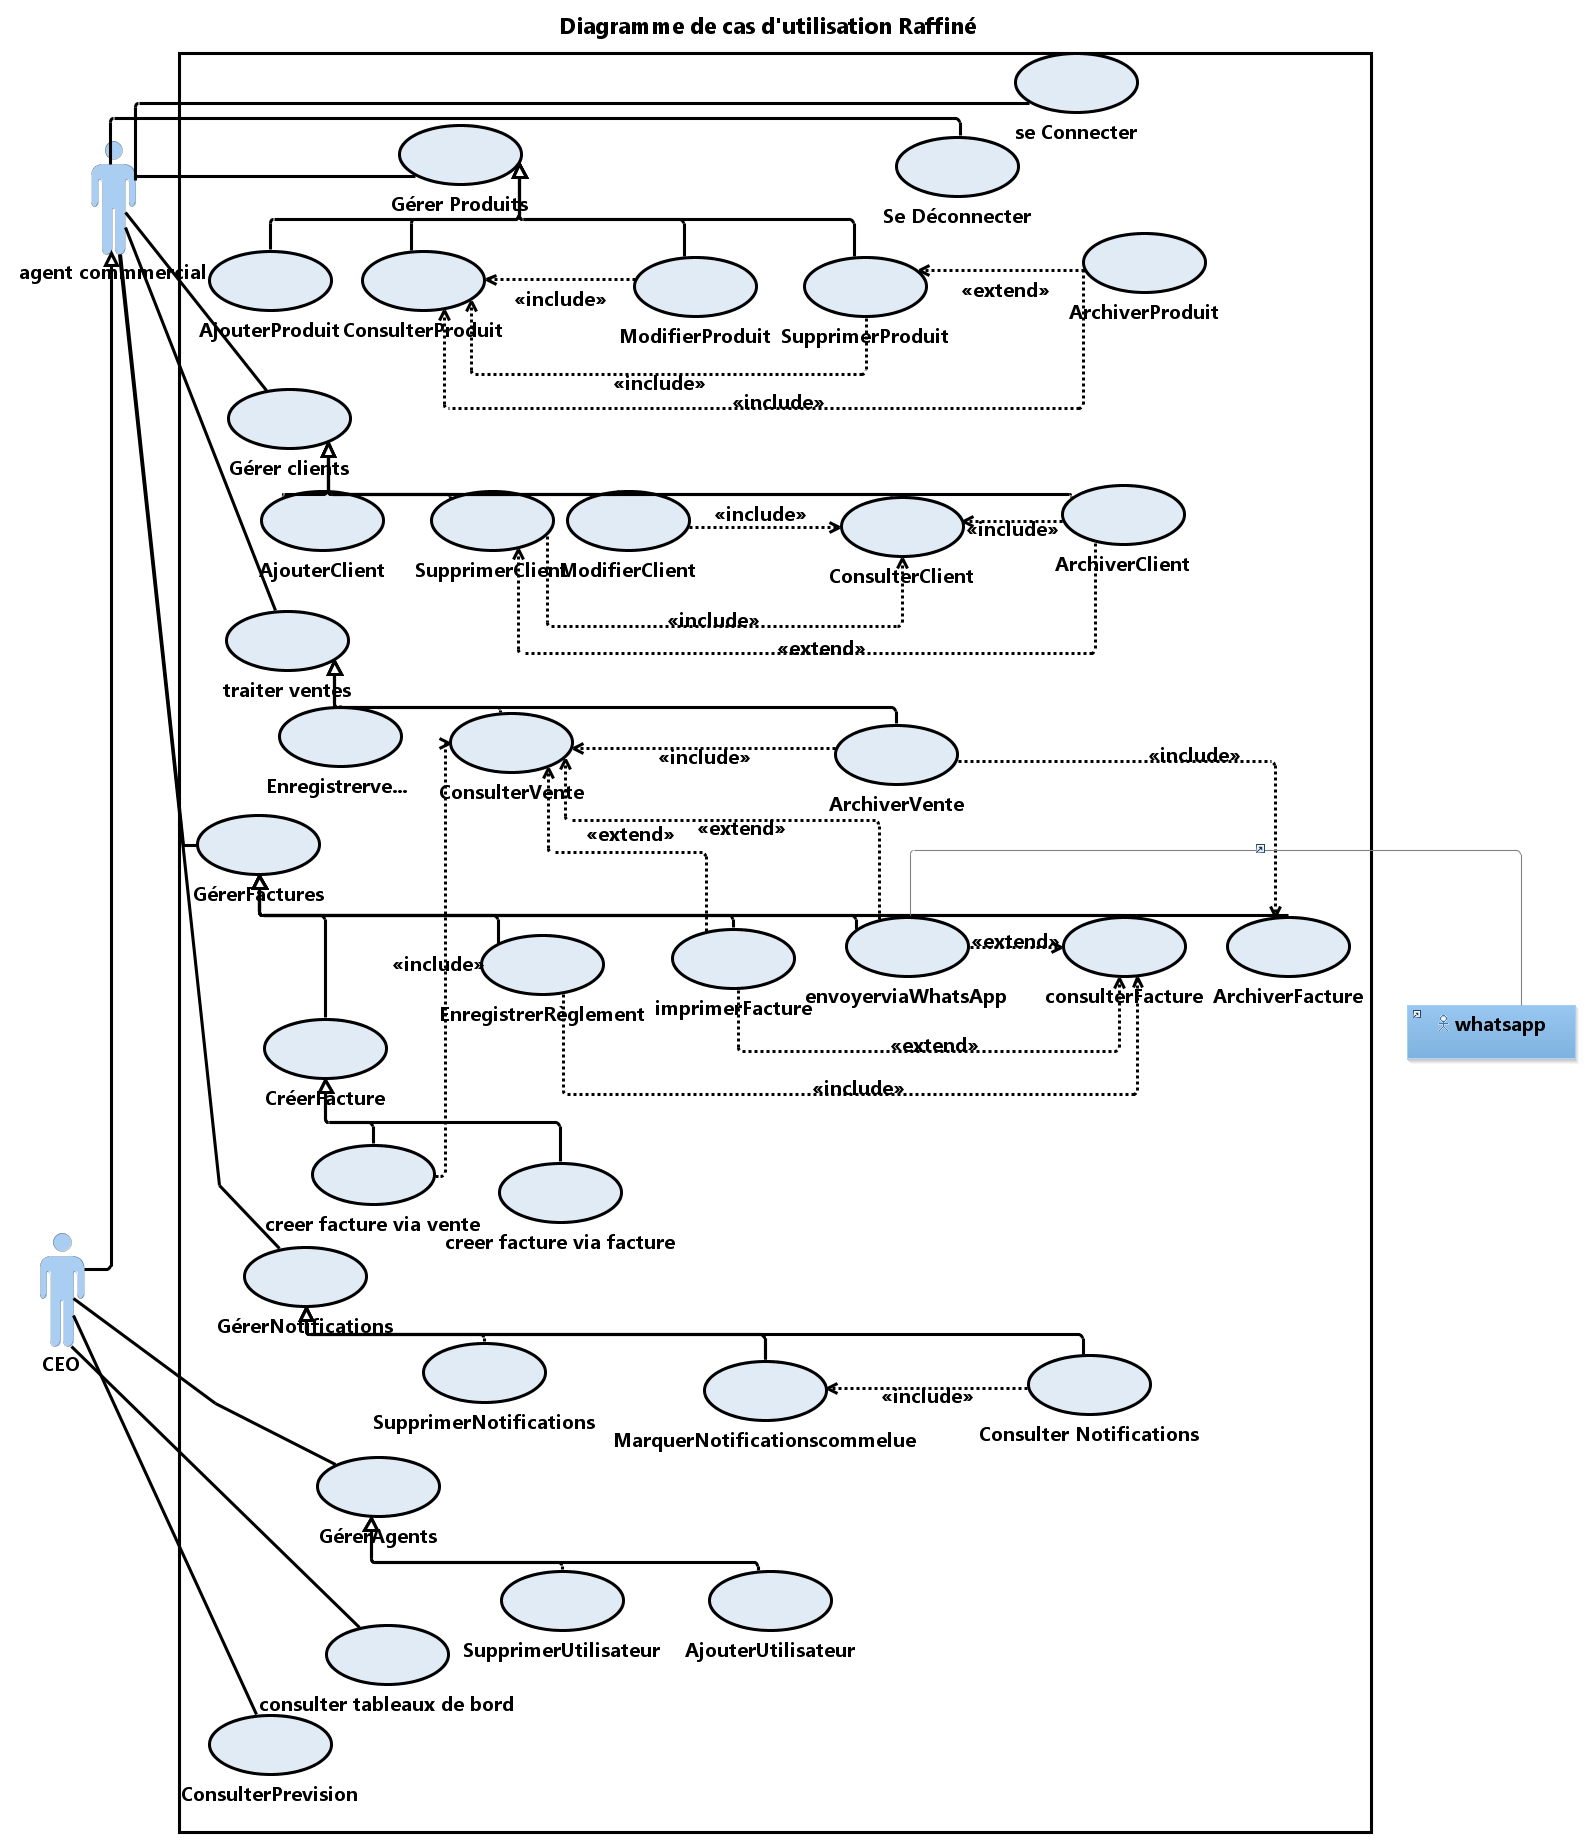
\includegraphics[width=1.3\textwidth, height=0.92\textheight, keepaspectratio]{images/MCU_DiagrammeCasUtilisationRaffiné.png}%
}
  \caption{Diagramme de cas d'utilisation raffiné}
  \label{fig:diagrammeUtilisationRaffine}
\end{figure}

\section*{Conclusion}
À la fin de ce chapitre, nous avons établi une vision claire et ordonnée  sur l'expression des besoins du système.
L'identification des acteurs, les besoins fonctionnels,non fonctionnels et décisionnels a mis en evidence la spécification 
des cas d'utilisation Grâce à leur utilisation, ils ont ensuite été en mesure de modéliser de manière précise les interactions entre les
acteur et le systéme 
Ces éléments sont la base sur laquelle la phase de conception  est présentée dans le chapitre qui suit.
